% Standalone source of the figure fig:tiling of the continuum-limit paper.
% Build: pdflatex fig_tiling.tex (or lualatex); the paper includes the PDF.
\documentclass[border=2pt]{standalone}
% Shared preamble of the continuum-limit paper's standalone figures.
\usepackage{amsmath,amssymb,bm}
\usepackage{tikz}
\usetikzlibrary{calc}
\newcommand{\bS}{\mathbf{S}}
\newcommand{\bG}{\mathbf{G}}
\newcommand{\bK}{\mathbf{K}}
\newcommand{\bP}{\mathbf{P}}
\newcommand{\sinc}{\operatorname{sinc}}

\begin{document}
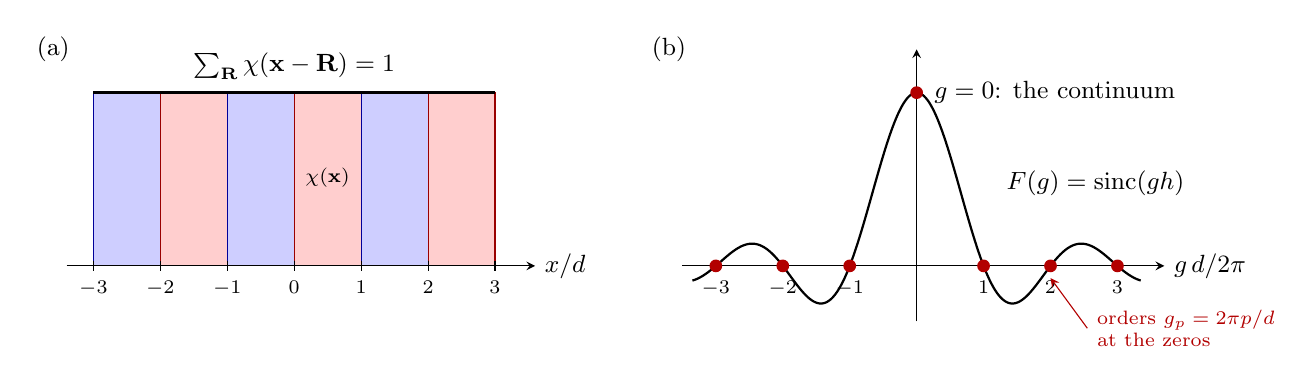
\begin{tikzpicture}[>=stealth, x=0.85cm, y=2.2cm, font=\small]
  % (a) the partition of unity: translated cube indicators sum to one
  \begin{scope}
    \foreach \k/\c in {-3/blue,-2/red,-1/blue,0/red,1/blue,2/red} {
      \fill[\c!55, opacity=0.35] (\k,0) rectangle (\k+1,1);
      \draw[\c!60!black] (\k,0) -- (\k,1) -- (\k+1,1) -- (\k+1,0);
    }
    \draw[->] (-3.4,0) -- (3.6,0) node[right] {$x/d$};
    \foreach \k in {-3,...,3} \draw (\k,0.03) -- (\k,-0.03) node[below, font=\scriptsize] {$\k$};
    \draw[very thick] (-3,1) -- (3,1);
    \node[above] at (0,1.02) {$\sum_{\mathbf R}\chi(\mathbf x-\mathbf R)=1$};
    \node[below, font=\scriptsize] at (0.5,0.62) {$\chi(\mathbf x)$};
    \node at (-3.6,1.25) {(a)};
  \end{scope}
  % (b) the same fact in Fourier space: the form factor vanishes on every reciprocal-lattice order but g = 0
  \begin{scope}[shift={(9.3,0)}]
    \draw[->] (-3.5,0) -- (3.7,0) node[right] {$g\,d/2\pi$};
    \draw[->] (0,-0.32) -- (0,1.25);
    \draw[thick, domain=-3.35:3.35, samples=301, smooth]
      plot (\x, {abs(\x) < 0.001 ? 1 : sin(180*\x)/(pi*\x)});
    \foreach \p in {-3,-2,-1,1,2,3} {
      \draw (\p,0.03) -- (\p,-0.03) node[below, font=\scriptsize] {$\p$};
      \fill[red!70!black] (\p,0) circle (2.3pt);
    }
    \fill[red!70!black] (0,1) circle (2.3pt);
    \node[right] at (0.12,1.0) {$g=0$: the continuum};
    \node[above right, align=left] at (1.2,0.35) {$F(g)=\sinc(gh)$};
    \draw[<-, red!70!black] (2,-0.07) -- (2.55,-0.36) node[right, align=left, font=\scriptsize]
      {orders $g_p=2\pi p/d$\\at the zeros};
    \node at (-3.7,1.25) {(b)};
  \end{scope}
\end{tikzpicture}
\end{document}
